Transformers operate on sequences of data $(x_{k})_{k=1}^n$, where $x_{k} \in \mathbb R^d$.
In the literature the elements of the input sequence are commonly referred to as tokens.
Central to Transformer models is the so-called attention mechanism.
The tokens $x_k$ are embedded into three different subspaces using linear mappings $Q, K, V \in \mathbb R^{d', d}$.
The mappings $Q$ and $K$ are used to compute the attention scores among the members of the sequence,
measuring the level of relevance of their respective information for each other

    \begin{equation} \label{eq:sa1}
        A_{ij} = \frac{\text{exp}(x_{i}^T K^T Q x_{j})}{\sum_{k = 1}^n \text{exp}(x_{k}^T K^T Q x_{j})} ~.
    \end{equation}

The outputs are then computed for all $j=1, ..., n$ by 

    \begin{equation} \label{eq:sa2}
        y_{j} = \sum_{i=1}^n A_{ij} V x_{i} ~.
    \end{equation}

Note that by construction for all $j = 1,..., n$ holds

    $$ \sum_{i=1}^n A_{ij} = 1 ~. $$

\begin{definition}[Self-Attention]
    Let $Q, K, V \in \mathbb R^{d', d}$.
    The operation described in equations (\ref{eq:sa1}), (\ref{eq:sa2}) 

        $$ \text{SA}: \mathbb R^{d} \times ... \times \mathbb R^{d} \to \mathbb R^{d} \times ... \times \mathbb R^{d} ~, ~~ \text{SA} (Q, K, V)(x_1, ..., x_k) = [y_1, ..., y_k] ~, $$

    is called self-attention.
\end{definition}

To increase the capacity of Transformer models, multiple self-attention operations, 
called heads in the literature, are used in parallel to process the input sequence.

\begin{definition}[Multi Headed Self-Attention]
    Let $Q_h, K_h, V_h \in \mathbb R^{d', d}$ for $h= 1,..., H$ and let $Q = (Q_1, ..., Q_H), K = (K_1, ..., K_H), V = (V_1, ..., V_H)$.
    The operation

        $$ \text{MSA}(Q, K, V) \left((x_{k})_{k=1}^n \right) = [\text{SA}(Q_1, K_1, V_1)\left((x_{k})_{k=1}^n \right), ..., \text{SA}(Q_H, K_H, V_H)\left((x_{k})_{k=1}^n \right)] ~, $$

    is called multi headed self-attention.
\end{definition}

\begin{figure}[h!]
    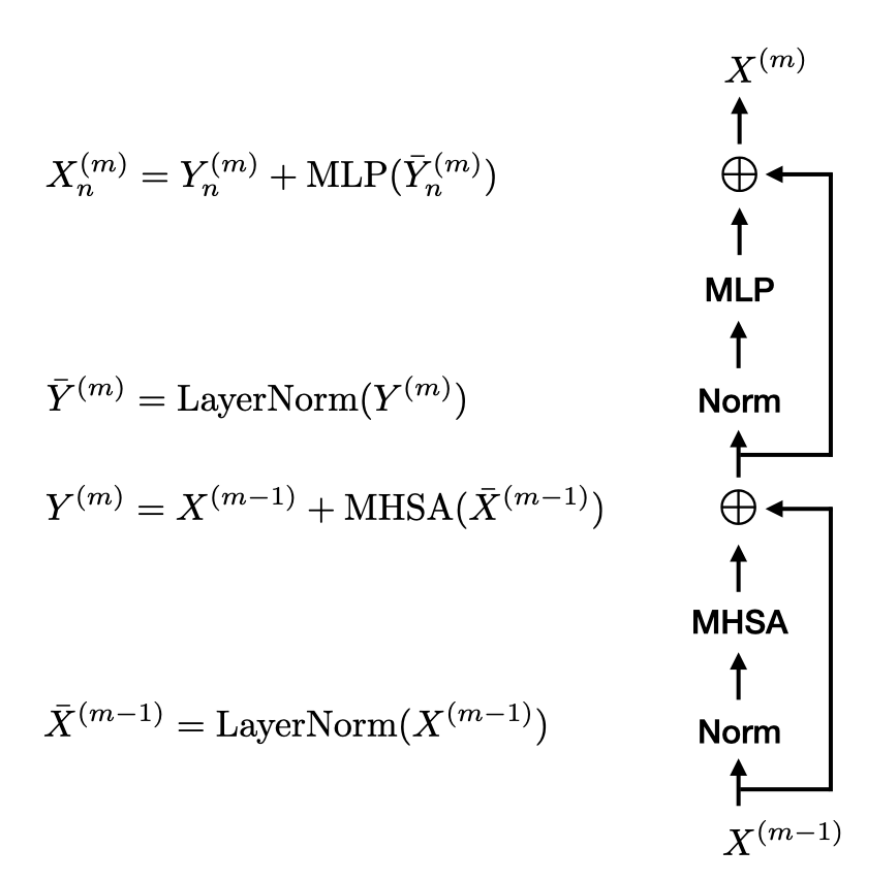
\includegraphics[width=0.6\textwidth]{models/preliminaries/imgs/transformer-block.png}
    \caption{Image taken from \cite{turnerIntroductionTransformers2024}, Transformer Block architecture.}
    \label{fig:transformer_block}
\end{figure}

In order to refer to the architecture,
that is Multi Headed Self-Attention with dimension $d \in \mathbb N$ and number of heads $H \in \mathbb N$,
whose weights are not fixed but subject to optimization, 
we write $\text{MSA}(d, H)$.

Given a number of heads $H \in \mathbb N$ generally the embedding dimension of each head is chosen as $\frac{d}{H}$.

Another key ingredient for Transformer models is layer normalization.

\begin{definition}[Layer Normalization]
    Let $\gamma \in \mathbb R$ and $\beta \in \mathbb R^d$. The operation given by

        $$\text{LN} : \mathbb R^d \to \mathbb R^d ~, ~~ 
        \text{LN}(x) = \gamma \bar{x} + \beta 
        \text{ where } \bar{x}_{ki} = \frac{1}{\sqrt{\text{var}(x_{k})}} (x_{ki} - \sum_{j=1}^d x_{kj})$$

    is called layer normalization.
\end{definition}

Typically Multi Headed Self-Attention is used in transformer blocks,
the architecture is outlined in figure \ref{fig:transformer_block}.

First layer normalization is applied to the inputs before the Multi Headed Self-Attention is being performed.
The input is then added back to the outputs via a residual connection.
The intermediate throughputs then undergo a second round of layer normalization, 
thereafter the tokens are processed individually by a neural network,
before a second residual connection adds the intermediate results to the outputs.
We describe this operation formally in the next definition.

\begin{definition}[Transformer Block] 
    \label{def:transformer_block}
    Let $d, H \in \mathbb N$ and $\Phi: \mathbb{R}^d \to \mathbb{R}^d$ be some mapping.
    The architecture 

        \begin{equation*}
            \Tau(d, H, \Phi) = R \big( \Phi \circ \text{LN} \big) \circ R \big( \text{MSA}(d, H) \circ \text{LN} \big)
        \end{equation*}

    is called a Transformer Block.
\end{definition}

Typically the mapping $\Phi$ is some neural network, with only a few number of layers.

Transformers operate on sequential data, 
so how to apply these models to images?
In their 2020 paper "An image is worth 16 $\times$ 16 words: Transformers for image recognition at scale",
Dosovitskiy et al. \cite{dosovitskiyImageWorth16x162021} propose to partition image data $X \in \mathbb R^{C \times H \times W}$
into a sequence of patches sized $P \times P$, for some $P \in \mathbb N$, 
which are flattened and then treated as tokens and fed to the transformer. 
More precisely the sequence is given by $(\hat{x}_k)_{k=1}^N$ where $\hat{x}_k \in \mathbb R^{C \cdot P^2}$ and $N = \frac{HW}{P^2}$.
Here we implicitly assume that $H \mod P = W \mod P = 0$, i.e. both the height and the width are devisable by the patch size $P$.
Let $w = \frac{W}{P}$, mathematically the partitioning can be described as follows 

    \begin{equation} \label{eq:vit_patch}
        \hat{x}_{k}(c_i \cdot h_i \cdot w_i) = X \left( c_i, \lfloor \frac{k}{w} \rfloor + h_i, k \mod w + w_i \right) ~,
    \end{equation}

for $k = 1, ..., N$, $c_i = 1, ..., C$ and $h_i, w_i = 1, ..., P$.
Lastly the flattened patches are embedded to obtain the final sequence of tokens $(x_k)_{k=1}^N$,
that is

    $$ x_k = E \hat{x}_k ~, $$

for some $E \in \mathbb R^{D \times C \cdot P^2}$.
The approach is also visualized in figure \ref{fig:vit}.

\begin{figure}[h!]
    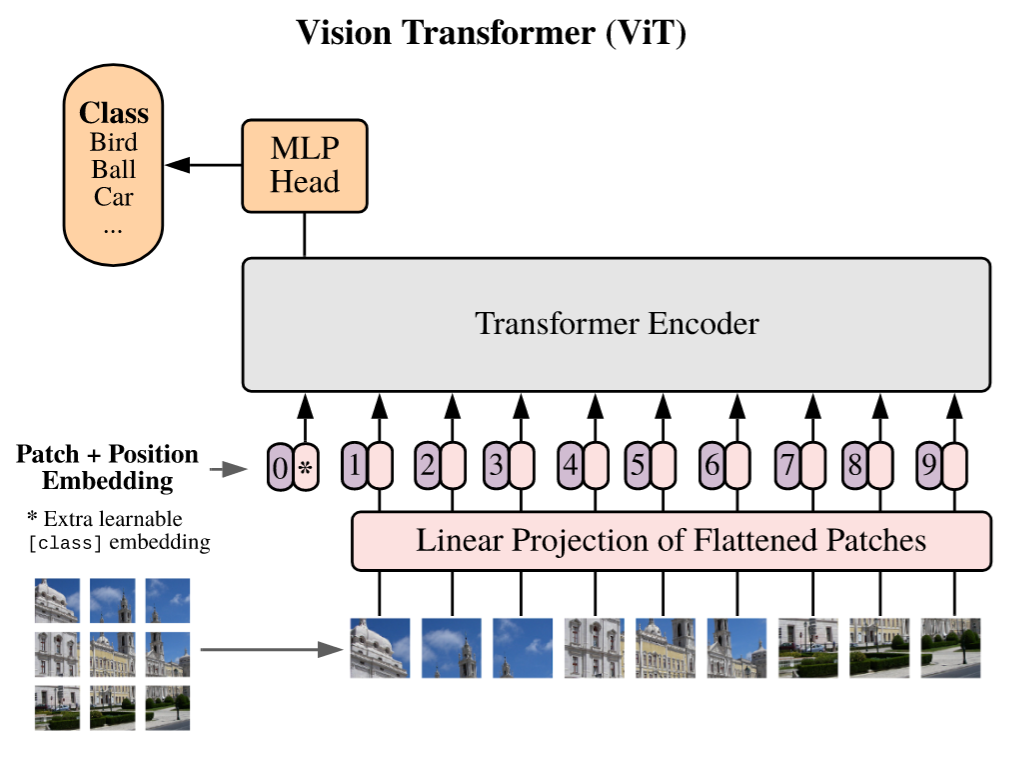
\includegraphics[width=0.6\textwidth]{models/preliminaries/imgs/vit.png}
    \caption{Image taken from \cite{dosovitskiyImageWorth16x162021}, Vision Transformer.}
    \label{fig:vit}
\end{figure}

A problem that comes with this approach, 
pointed out by Liu et al. \cite{liuSwinTransformerHierarchical2021}
that unlike in language, where a word naturally offers itself as the atomic unit,
visual elements vary in scale,
making the fixed patch sizes unsuitable for tasks requiring predictions at pixel level,
as for example semantic segmentation. 
Simply treating each individual pixel as a token would solve the problem,
but at the same time introduce immense computational complexity.
For a full HD image of size $1920 \times 1080$ this leads to a sequence length of $2.0736 \cdot 10^{6}$.
Thus to reduce computational complexity,
but at the same time maintain a global receptive field, Liu et al. \cite{liuSwinTransformerHierarchical2021} propose three concepts.

First the image is partitioned into non-overlapping patches,
similarly as described in equation (\ref{eq:vit_patch}),
with the difference being that each pixel within the patch is treated as a token itself

    \begin{equation} \label{eq:swin_partitioning}
        x_{i \cdot j}^{(p)}(c) = X \left( c, \left\lfloor \frac{p}{P} \right\rfloor + i, p \mod P + j \right) ~,
    \end{equation}

where $p = 1, ..., N$ and $i, j = 1, ..., P$. 
Self-attention is then performed locally inside of the patch, 
that is

    \begin{equation} \label{eq:swin1}
        (y_{k}^{(p)})_{k=1}^P = \text{MSA}(Q, K, V) \left( (x_{k}^{(p)})_{k=1}^P \right) ~,
    \end{equation}

for $p = 1, ..., N$, for some $Q, K, V \in \mathbb R^{H \times \frac{d}{H} \times d}$.

If equation (\ref{eq:swin1}) would be used repeatedly to update features,
information is limited to flow only inside the individual patches. 
To this end Liu et al. \cite{liuSwinTransformerHierarchical2021} introduce the shifted window mechanism.
Consecutive operations of self-attention use different partitionings of the feature map.
We consider the partitioning described in equation (\ref{eq:swin_partitioning}) as the unshifted variant,
for the shifted partitioning the borders of the patches are moved down and to the right by $s = \left \lfloor \frac{P}{2} \right \rfloor$ units,
that is

    \begin{equation*}
        x_{i \cdot j}^{(p)}(c) = X \left( c, \left(\left\lfloor \frac{p}{P} \right\rfloor + i + s \right) \mod H, \left( p \mod P + j + s \right) \mod W \right) ~,
    \end{equation*}

where $p = 1, ..., N$ and $i, j = 1, ..., P$. 
Applying the modulo to the arguments, leads to a cyclic shift, visualized in figure \ref{fig:cyclic_shift}.
This is necessary as the shift leads to overshooting the margins of the feature map.
Instead also padding techniques could be applied,
but Liu et al. \cite{liuSwinTransformerHierarchical2021} report achieving better results, 
whilst saving computational complexity.

\begin{figure}[h!]
    \begin{center}
        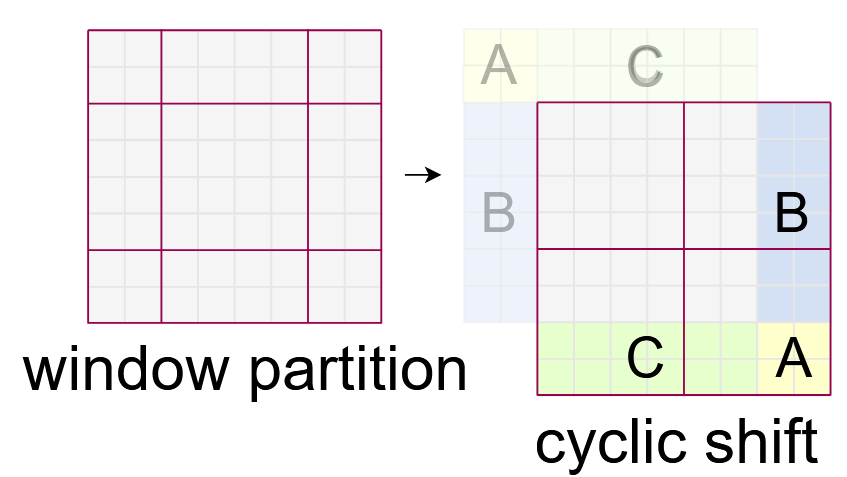
\includegraphics[width=0.6\textwidth]{models/preliminaries/imgs/cyclic-shift.png}
    \end{center}
    \caption{Image taken from \cite{liuSwinTransformerHierarchical2021}, visualizing the cyclic shift.
        Here the pixels in the image are rearranged, and then the unshifted partitioning is used, to obtain the cyclic shift.}
    \label{fig:cyclic_shift}
\end{figure}

To enable a global receptive field, 
Liu et al. \cite{liuSwinTransformerHierarchical2021} propose to merge neighboring patches, 
after the inputs are processed by a certain number of SWin TransformerBlocks.
To this end patches $P_1, ..., P_4 \in \mathbb R^{C \times P \times P}$,
inside a neighborhood of size $2 \times 2$ are stacked along the channel dimension,
to form a super patch $\hat{P} = [P_1, ..., P_4] \in \mathbb R^{4 \cdot C \times P \times P}$.
To fuse the features a convolutional layer is applied halving the channel dimension of the super patch

    \begin{equation*}
        P = C(4 \cdot C, 2 \cdot C, \text{kernel-size}=3, \text{padding}=1)(\hat{P}) ~.
    \end{equation*}

This process is repeated until the entire feature map is of size $P \times P$.
The overall architecture of the SWin Transformer is shown in figure \ref{fig:swin}.

\begin{figure}[h!]
    \begin{center}
        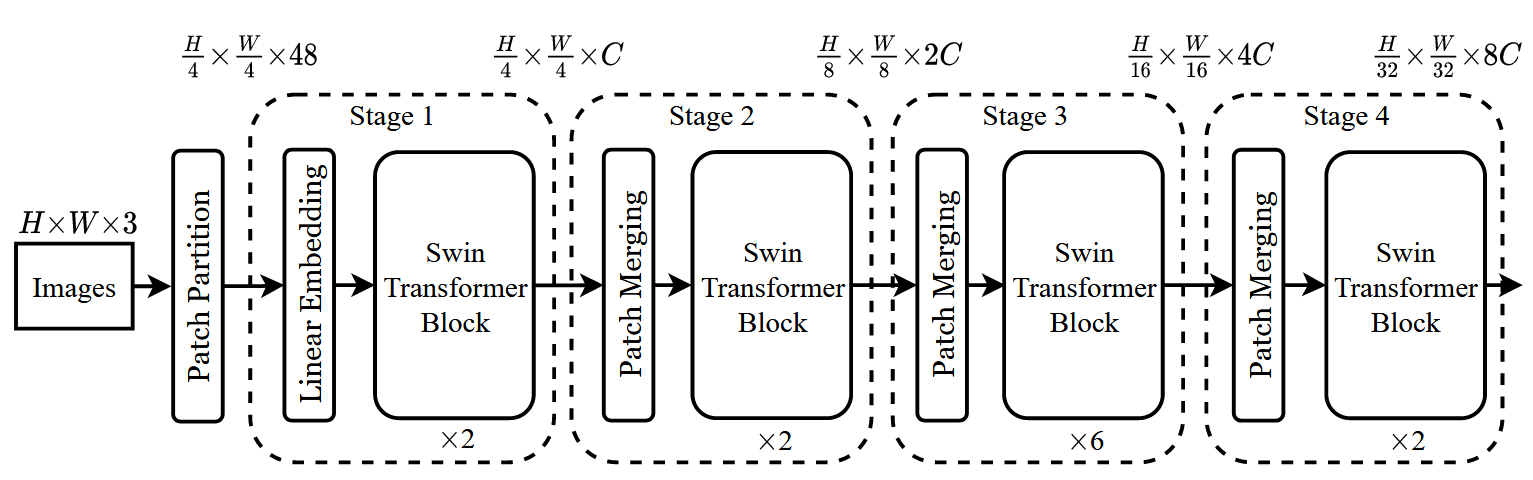
\includegraphics[width=0.6\textwidth]{models/preliminaries/imgs/swin.png}
    \end{center}
    \caption{Image taken from \cite{liuSwinTransformerHierarchical2021}, SWin Transformer.}
    \label{fig:swin}
\end{figure}

\begin{definition}[Shifted window Transformer Block]
    Let $d, H \in \mathbb N$ and $\Phi: \mathbb R^d \to \mathbb R^{d}$
\end{definition}

Chen et al. \cite{chenHATHybridAttention2024} introduce overlapping Cross Attention (OCA),
a modification of SWin Transformers.
Whilst in equation (\ref{eq:swin_partitioning}) the patches where constructed to partition the feature map,


